%!TEX program = xelatex
\documentclass[cn,hazy,pku,12pt,normal,math=newtx,cite=super]{elegantnote}
\title{双液体系沸点-成分图的绘制}

\author{刘松瑞 \quad 2100011819 \\ 组号:24 \quad 组内编号:5}
\institute{化学与分子工程学院}

\expdate{\zhdate{2023/11/9}}
\temperature{18.4 \si{^{\circ}C}}
\pressure{102.98 \si{kPa}}

\usepackage{gensymb}
\usepackage{array}
\usepackage{subfigure}
\usepackage[fontset=windows]{ctex}
\usepackage{graphicx}
\usepackage{float}
\usepackage{caption}
\usepackage{multirow}
%\usepackage{subfig}
%\usepackage{float}
\begin{document}

\maketitle

\keywords{双液系 \quad 乙醇-环己烷 \quad 相图 \quad 阿贝折射仪}

\abstracts{
    本实验通过配制不同浓度的乙醇-环己烷的标准溶液,测量了乙醇-环己烷双液系的工作曲线,
    并通过测量乙醇-环己烷恒沸体系气相和液相的沸点与折射率,从而确定其质量分数,绘制了乙醇-环己烷双液系的相图,
    求得这个体系的最低恒沸点为 64.31 $\degree C$,对应的乙醇的质量分数为 0.3123,与文献值接近。
}

\newpage


\section{引言}

\subsection{实验目的与原理}

实验目的与原理详见预习报告图~\ref{1}。 \cite{pcl2002}

\begin{figure}[htbp]
    \centering
    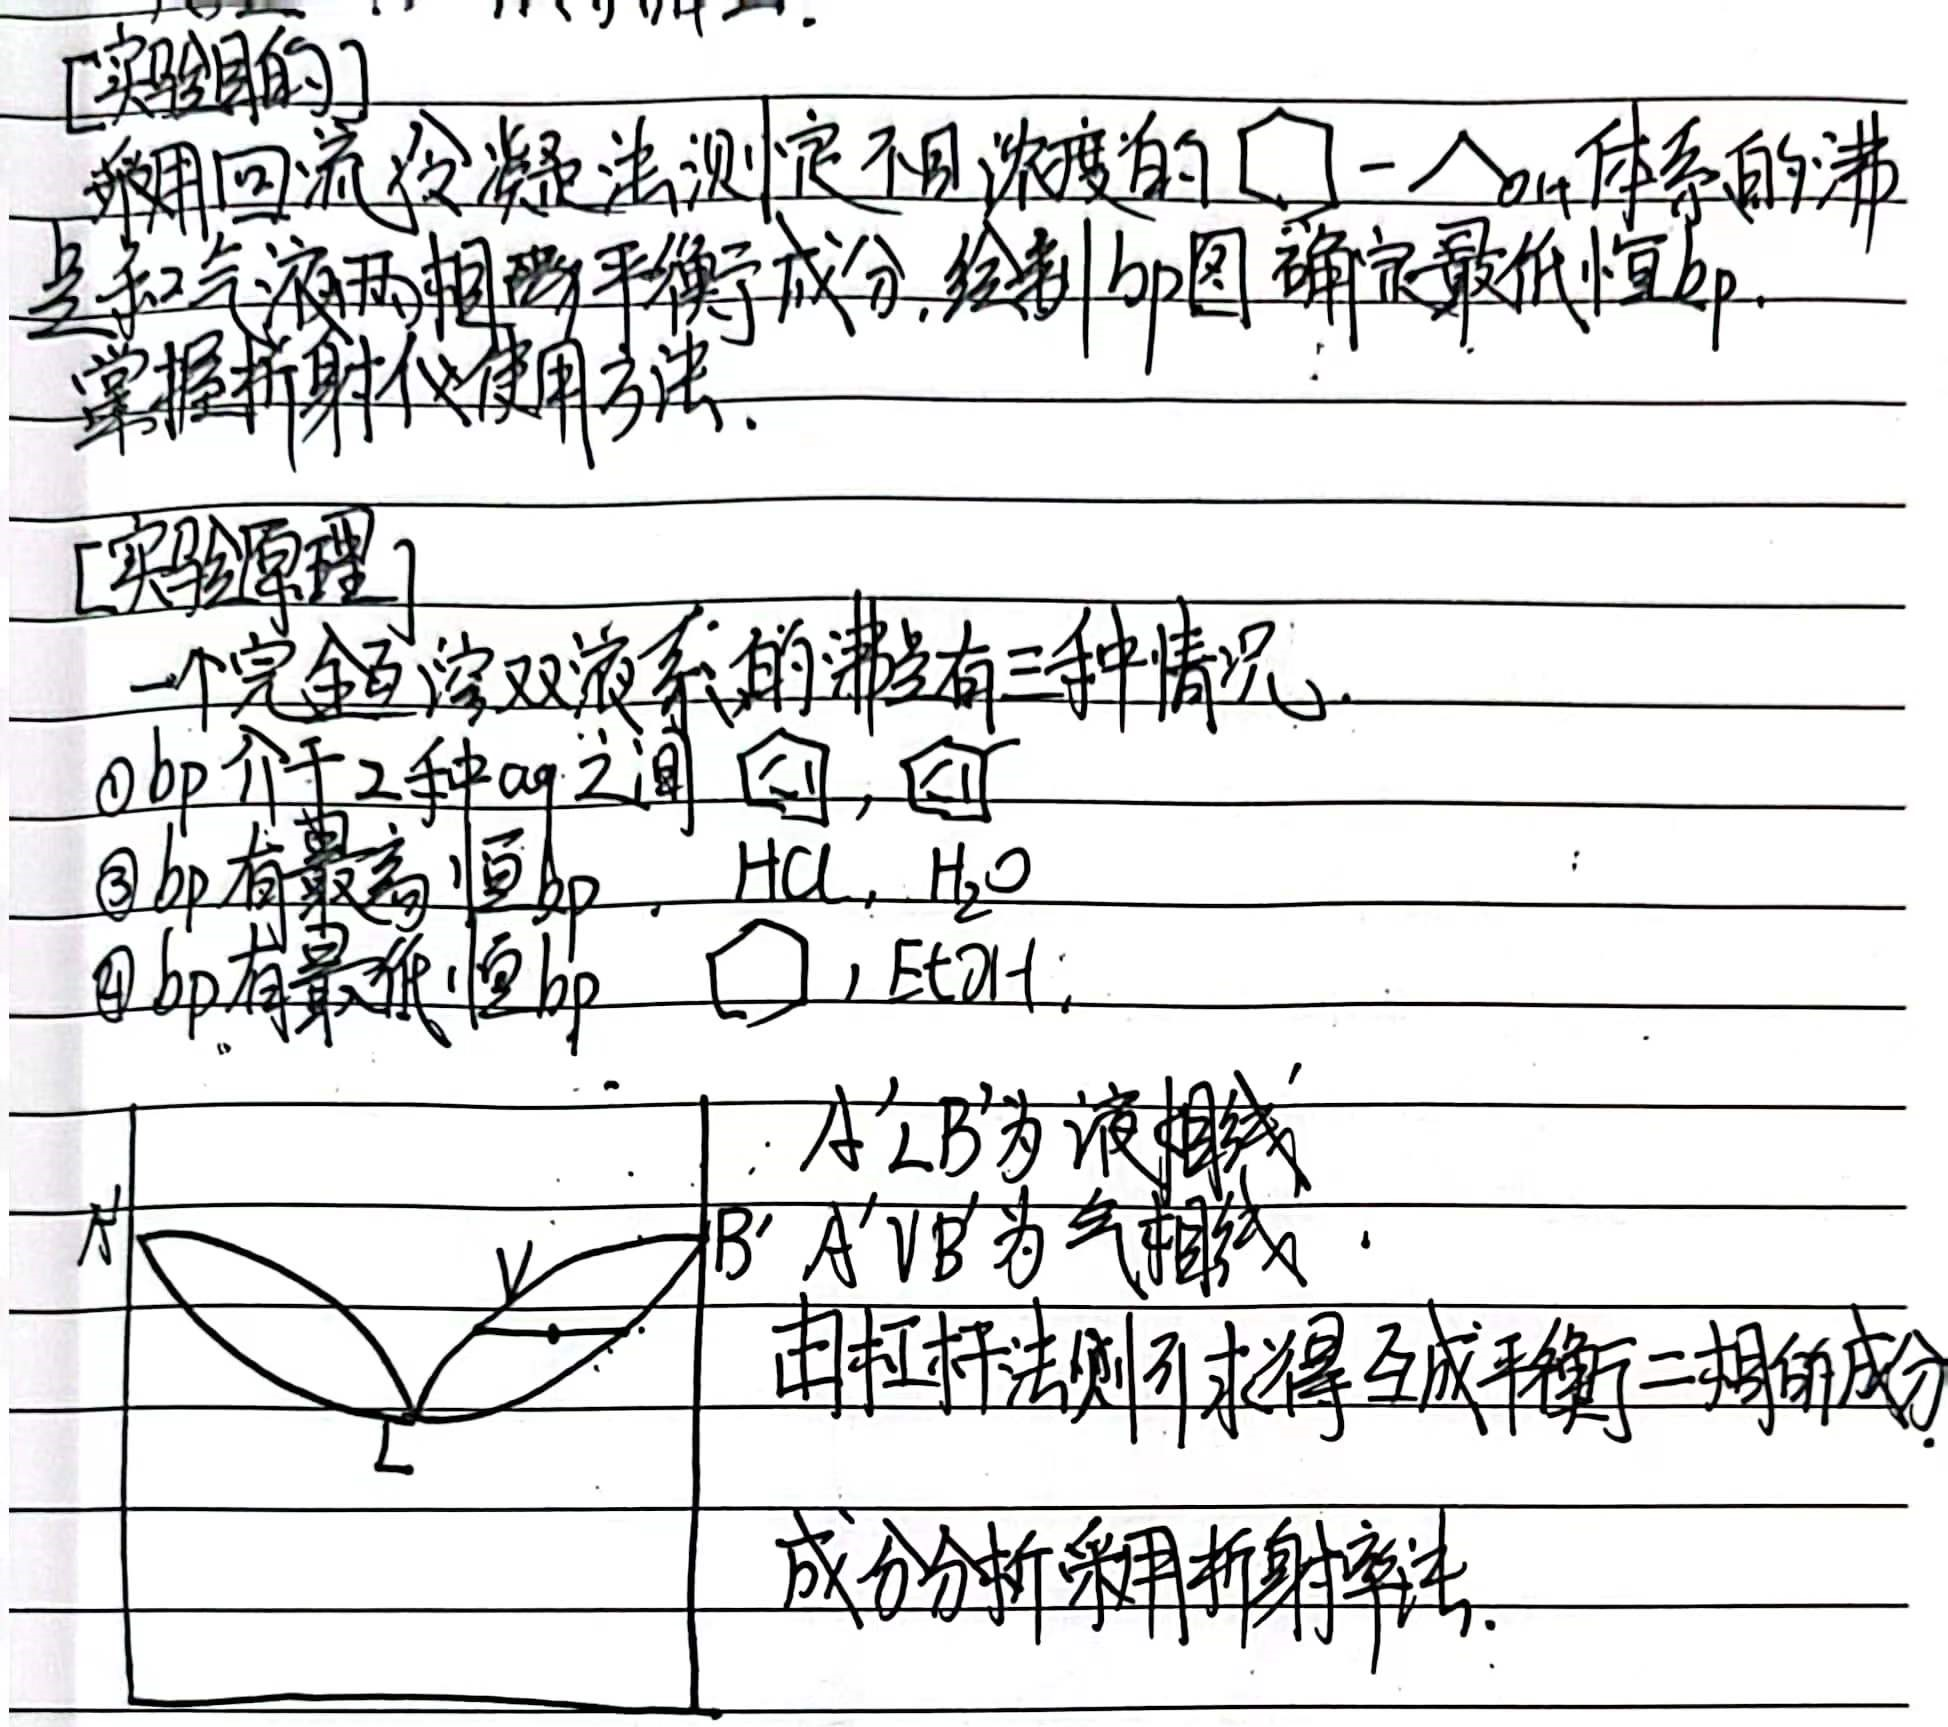
\includegraphics[width = .70\textwidth]{image/yxbg_1.jpg}
    \caption{实验的目的与原理}\label{1}
\end{figure}

\subsection{实验方法}

使用恒沸点仪,阿贝折射仪测定在不同比例的环己烷与乙醇溶液的沸点,绘制双液系沸点-成分图。


\section{实验部分}

\subsection{实验步骤}

实验步骤详见预习报告图 \ref{b} 和图 \ref{a} 。
\begin{figure}[htbp]
    \centering
    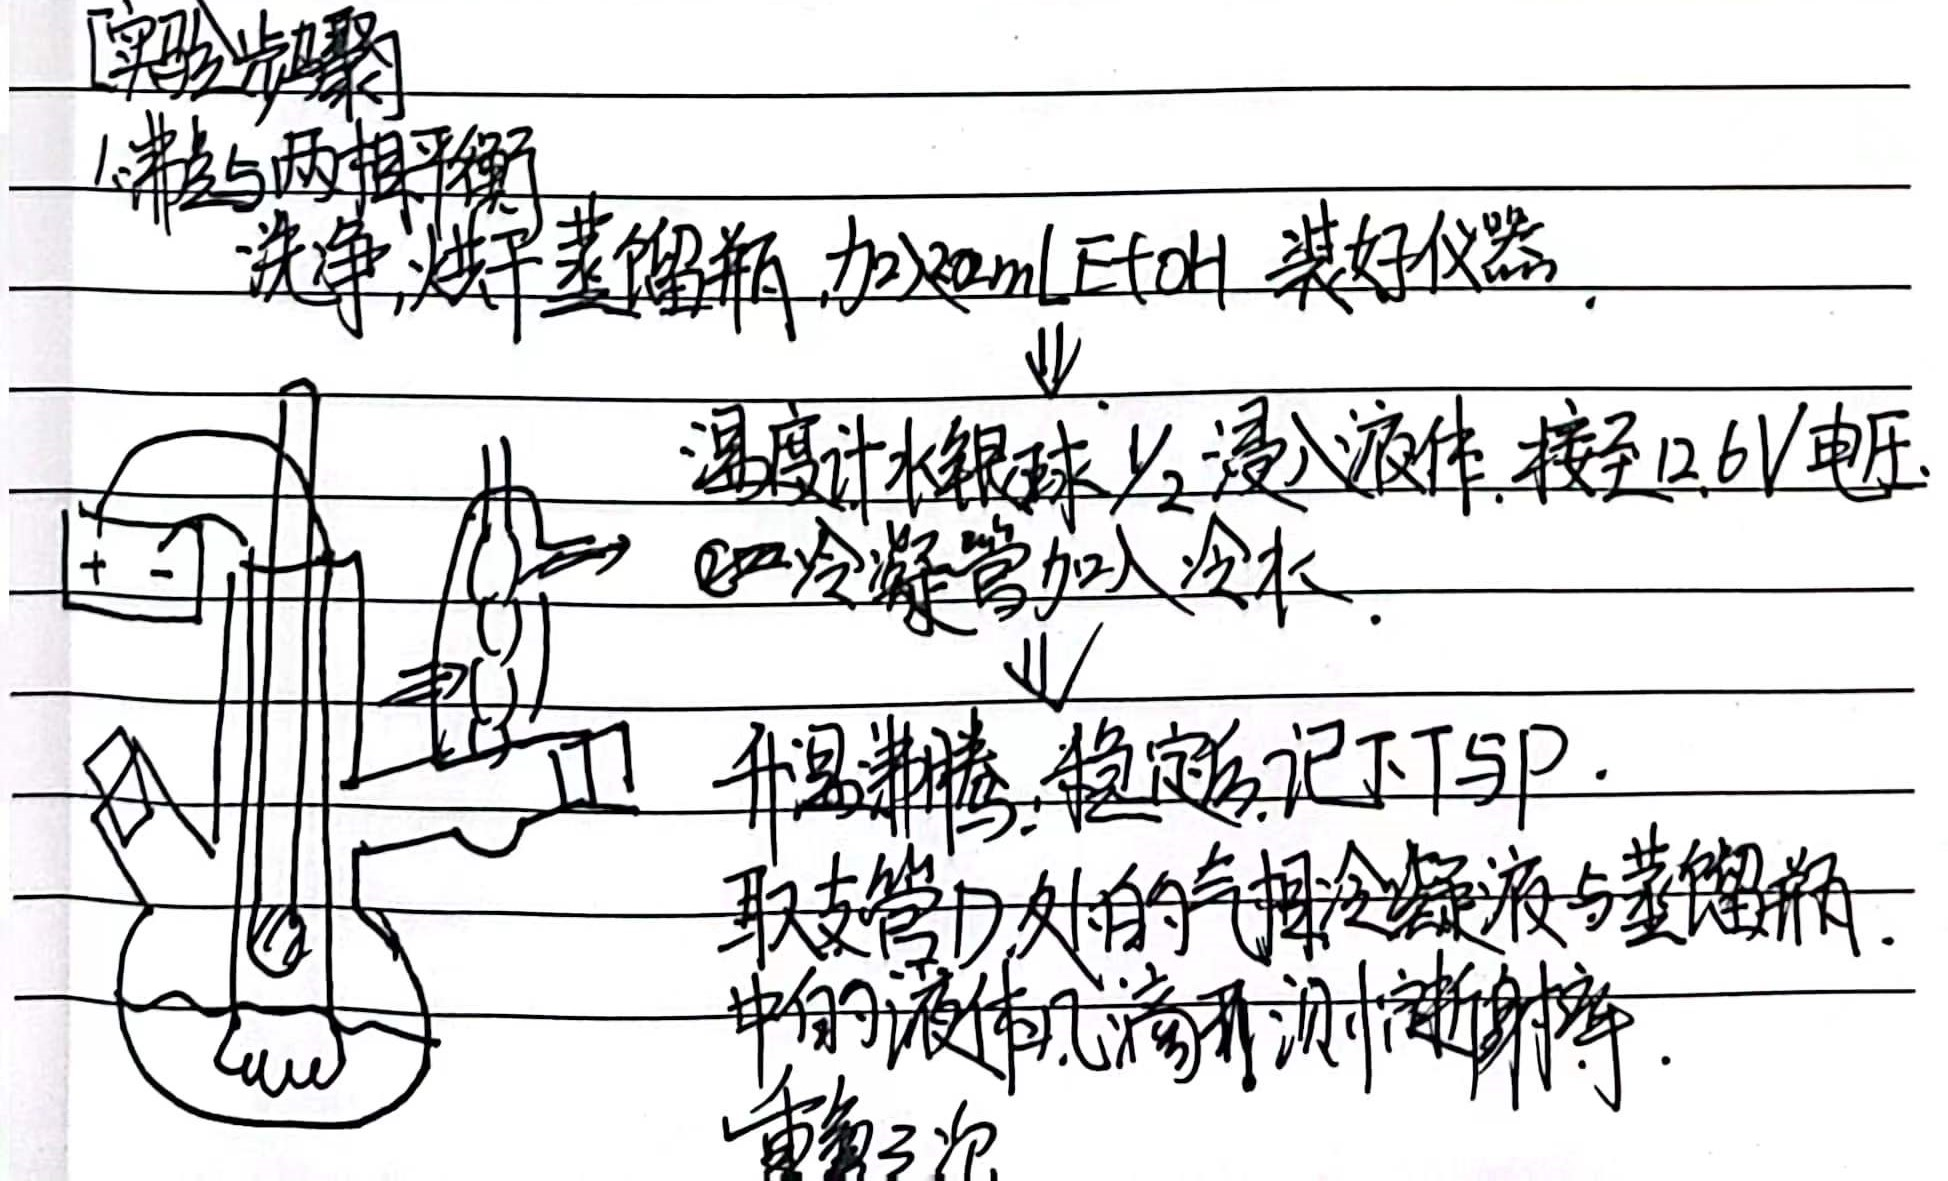
\includegraphics[width = .70\textwidth]{image/yxbg_2.jpg}
    \caption{实验步骤}\label{b}
\end{figure}

\begin{figure}[htbp]
    \centering
    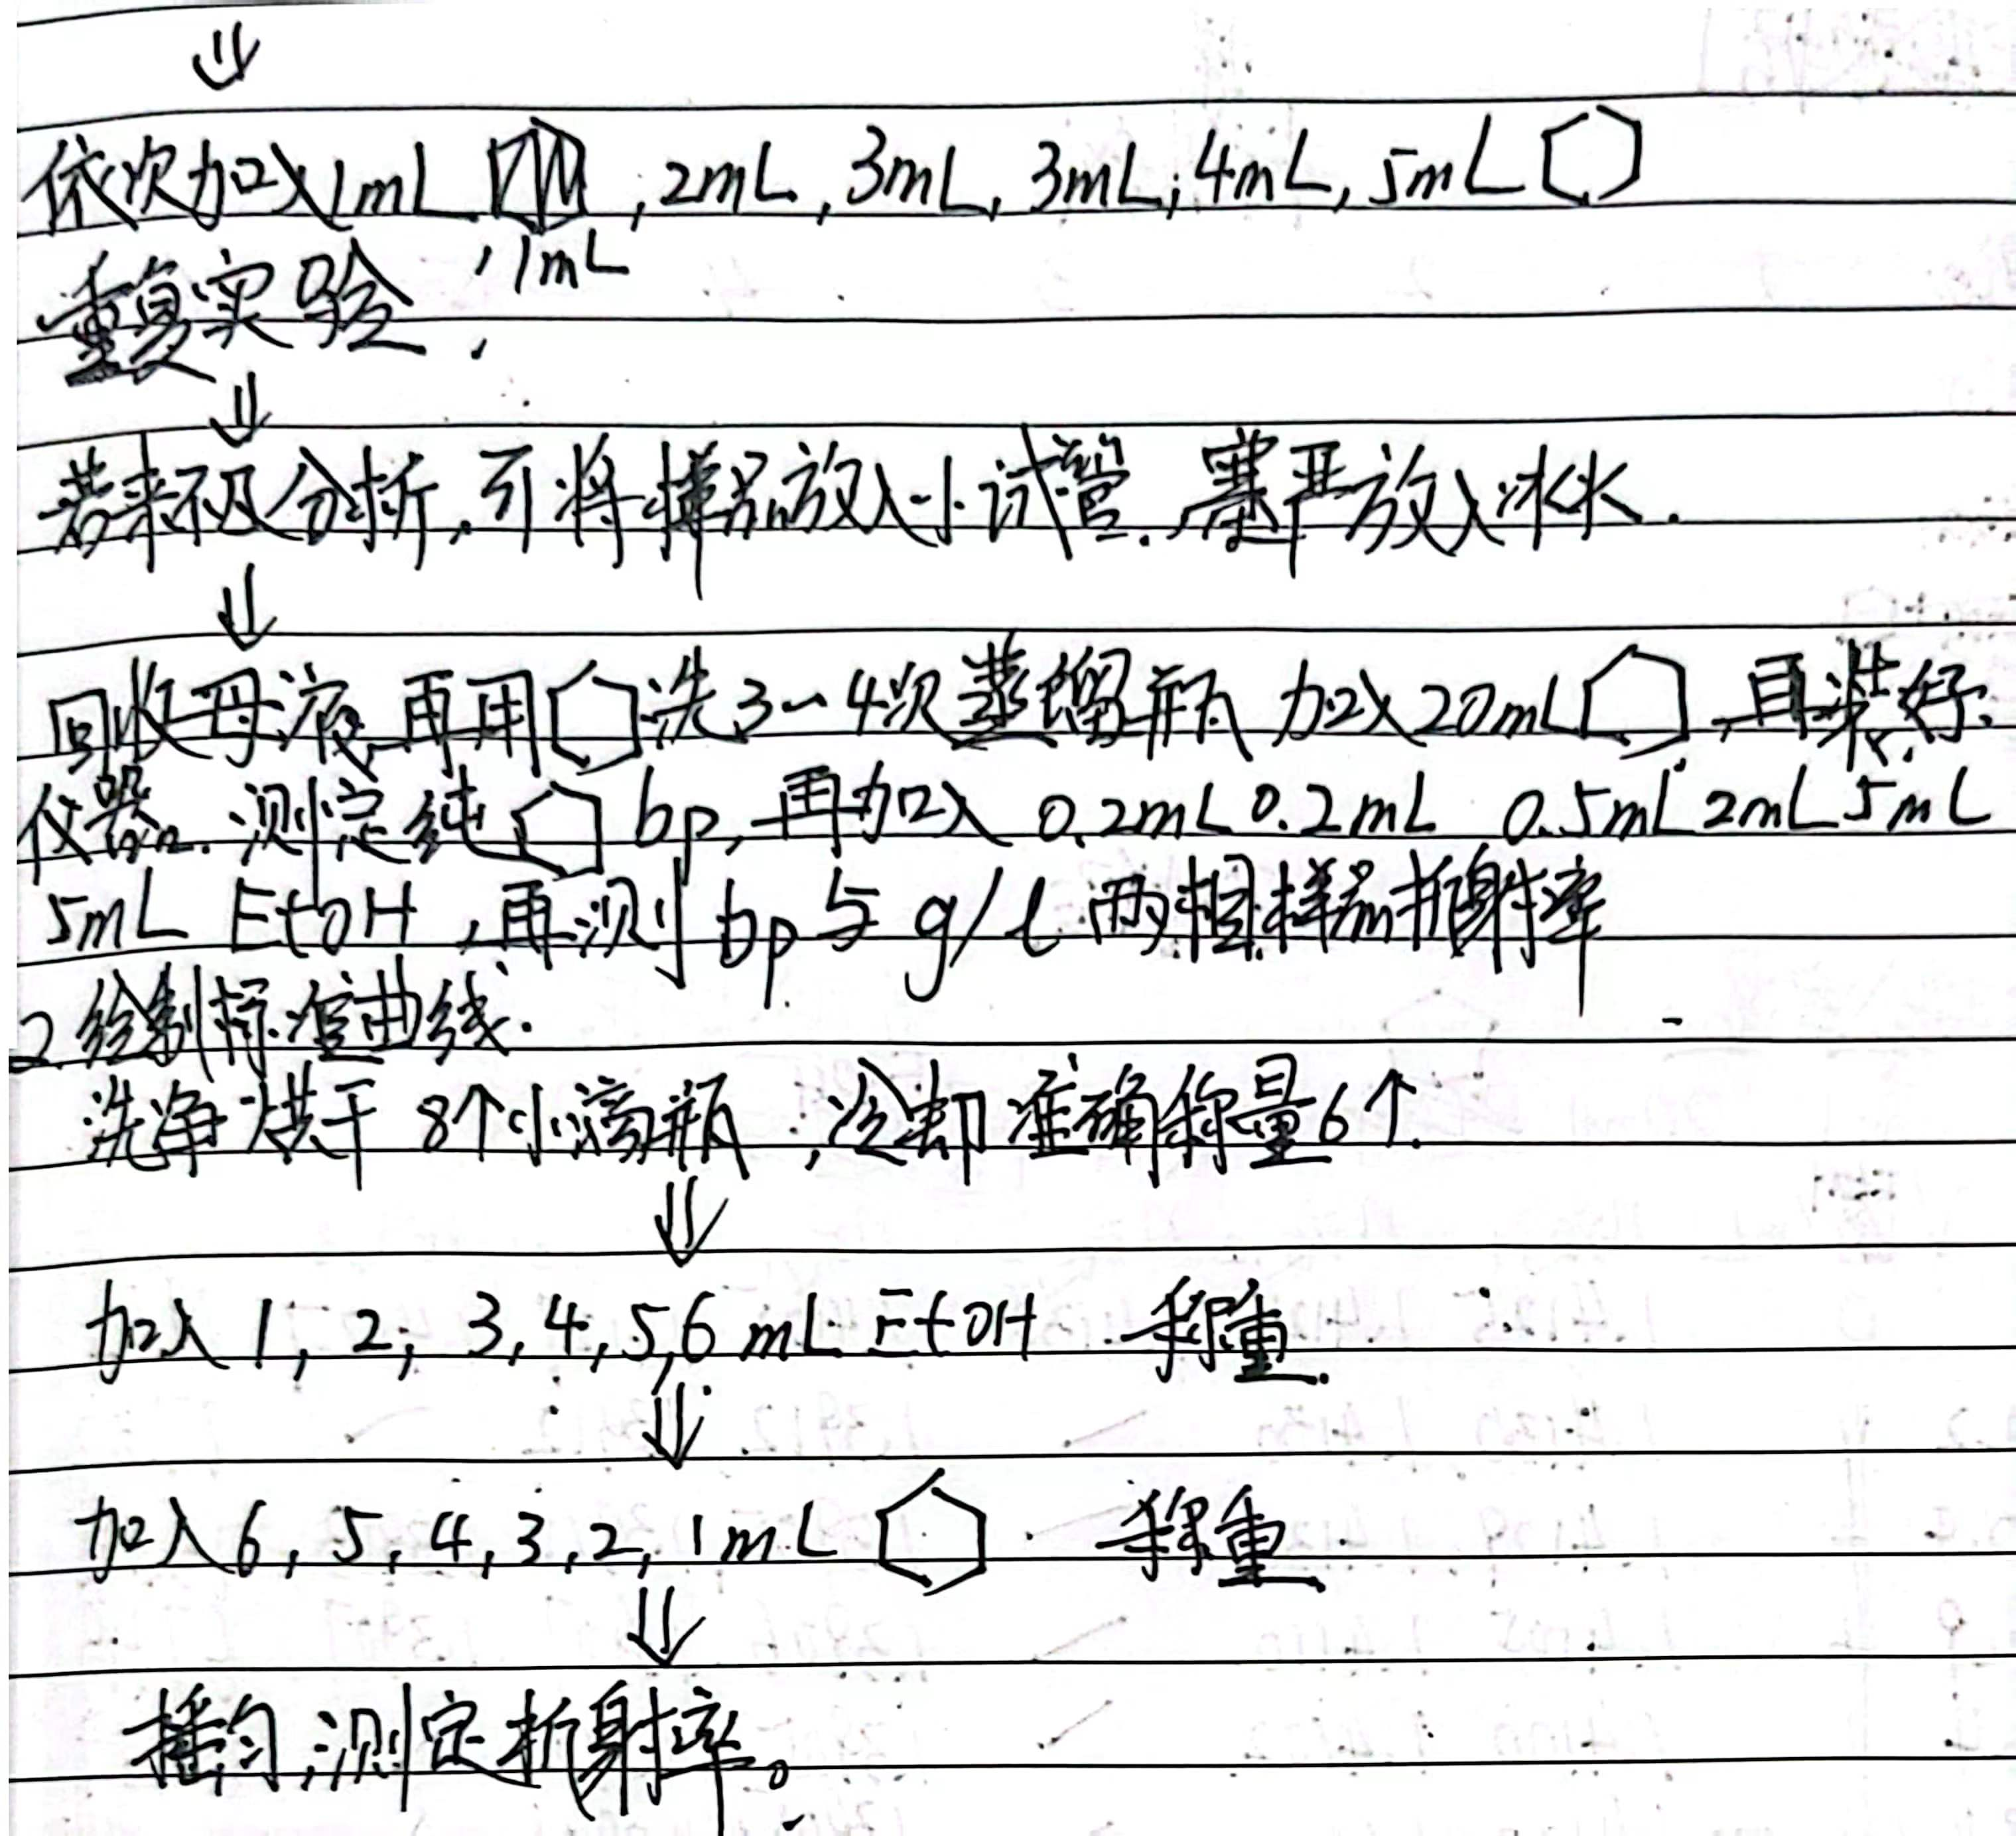
\includegraphics[width = .70\textwidth]{image/yxbg_3.jpg}
    \caption{实验步骤}\label{a}
\end{figure}

\subsection{仪器与药品}

\begin{enumerate} %有序列表
    \item 试剂 \\   环己烷(AR),无水乙醇(AR),丙酮(AR)。

    \item 仪器 \\   恒沸点仪,阿贝折射仪,温度测定及加热控制装置,导线,30 mL 滴瓶(公用),1、
    2、5 和 20 mL 移液管各两只,滴管。
\end{enumerate}

\section{实验现象与数据处理}
\subsection[short]{绘制标准曲线}

在 29.9$\rm \degree C$ 下,纯组分的折射率测定结果如表 \ref{01},不同成分标准溶液的质量与折射率的测定结果如表 \ref{02}。

\begin{table}[h]
    \centering
    \caption{纯组分的折射率}
    \label{01}
    \begin{tabular}{ccccc}
    \hline
    次数         & 1      & 2      & 3      & 平均     \\ \hline
    $n_{EtOH}$ & 1.3494 & 1.3495 & 1.3493 & 1.3494 \\
    $n_{Cy}$   & 1.4132 & 1.4130 & 1.4131 & 1.4131 \\ \hline
    \end{tabular}
\end{table}

\begin{table}[h]
    \centering
    \caption{不同成分标准溶液的质量}
    \label{02}
    \begin{tabular}{ccccccccccc}
    \hline
    $V_{EtOH}$/mL & $V_{Cy}$/mL & $m_{bottle}$/g & $m_{bottle+EtOH}$/g & $m_{bottle+EtOH+Cy}$/g & $\omega_{EtOH}$ \\ \hline
    1          & 8        & 28.6165    & 29.3876      & 35.5713          & 0.1109              \\
    2          & 7        & 28.9018    & 30.4918      & 35.8657          & 0.2283              \\
    3          & 6        & 33.3803    & 35.8620      & 40.5020          & 0.3485              \\
    4          & 5        & 35.5137    & 38.6506      & 42.5012          & 0.4489              \\
    5          & 4        & 27.3403    & 31.2458      & 34.3420          & 0.5578              \\
    6          & 3        & 32.6657    & 37.3899      & 39.6904          & 0.6725              \\
    7          & 2        & 32.0160    & 37.4172      & 38.9588          & 0.7780              \\
    8          & 1        & 32.2458    & 38.5282      & 39.2967          & 0.8910              \\ \hline
    \end{tabular}
\end{table}

\begin{table}[h]
    \centering
    \caption{不同成分标准溶液的折射率}
    \label{03}
    \begin{tabular}{cccccc}
    \hline
    $V_{EtOH}$/mL & $V_{Cy}$/mL & $n_{1}$ & $n_{2}$ & $n_{3}$ & $\bar{n}$ \\ \hline
    1          & 8        & 1.4046  & 1.4048  & 1.4047  & 1.4047    \\
    2          & 7        & 1.3963  & 1.3965  & 1.3962  & 1.3963    \\
    3          & 6        & 1.3879  & 1.3878  & 1.3880  & 1.3879    \\
    4          & 5        & 1.3810  & 1.3808  & 1.3809  & 1.3809    \\
    5          & 4        & 1.3732  & 1.3732  & 1.3735  & 1.3733    \\
    6          & 3        & 1.3670  & 1.3670  & 1.3671  & 1.3670    \\
    7          & 2        & 1.3610  & 1.3611  & 1.3610  & 1.3610    \\
    8          & 1        & 1.3595  & 1.3594  & 1.3596  & 1.3595    \\ \hline
    \end{tabular}
\end{table}

由文献可知,标准溶液的质量分数与折射率的关系可使用三次方程 \cite{2003}、六次方程 \cite{zgy}等高次方程描述,但是由于本次实验数据较少,若使用高次方程拟合会导致出现过拟合现象
因此选用二次多项式拟合标准溶液的质量分数与折射率的关系,得到结果如图 \ref{3} ,拟合曲线方程如下
$$
\bar{n} =   (1.4133 \pm 0.0012) + (-0.080 \pm 0.006) \cdot \omega_{\rm EtOH}  + (0.018 \pm 0.005) \cdot \omega_{\rm EtOH} ^2 \quad R^2 = 0.995
$$

\begin{figure}[htbp]
    \centering
    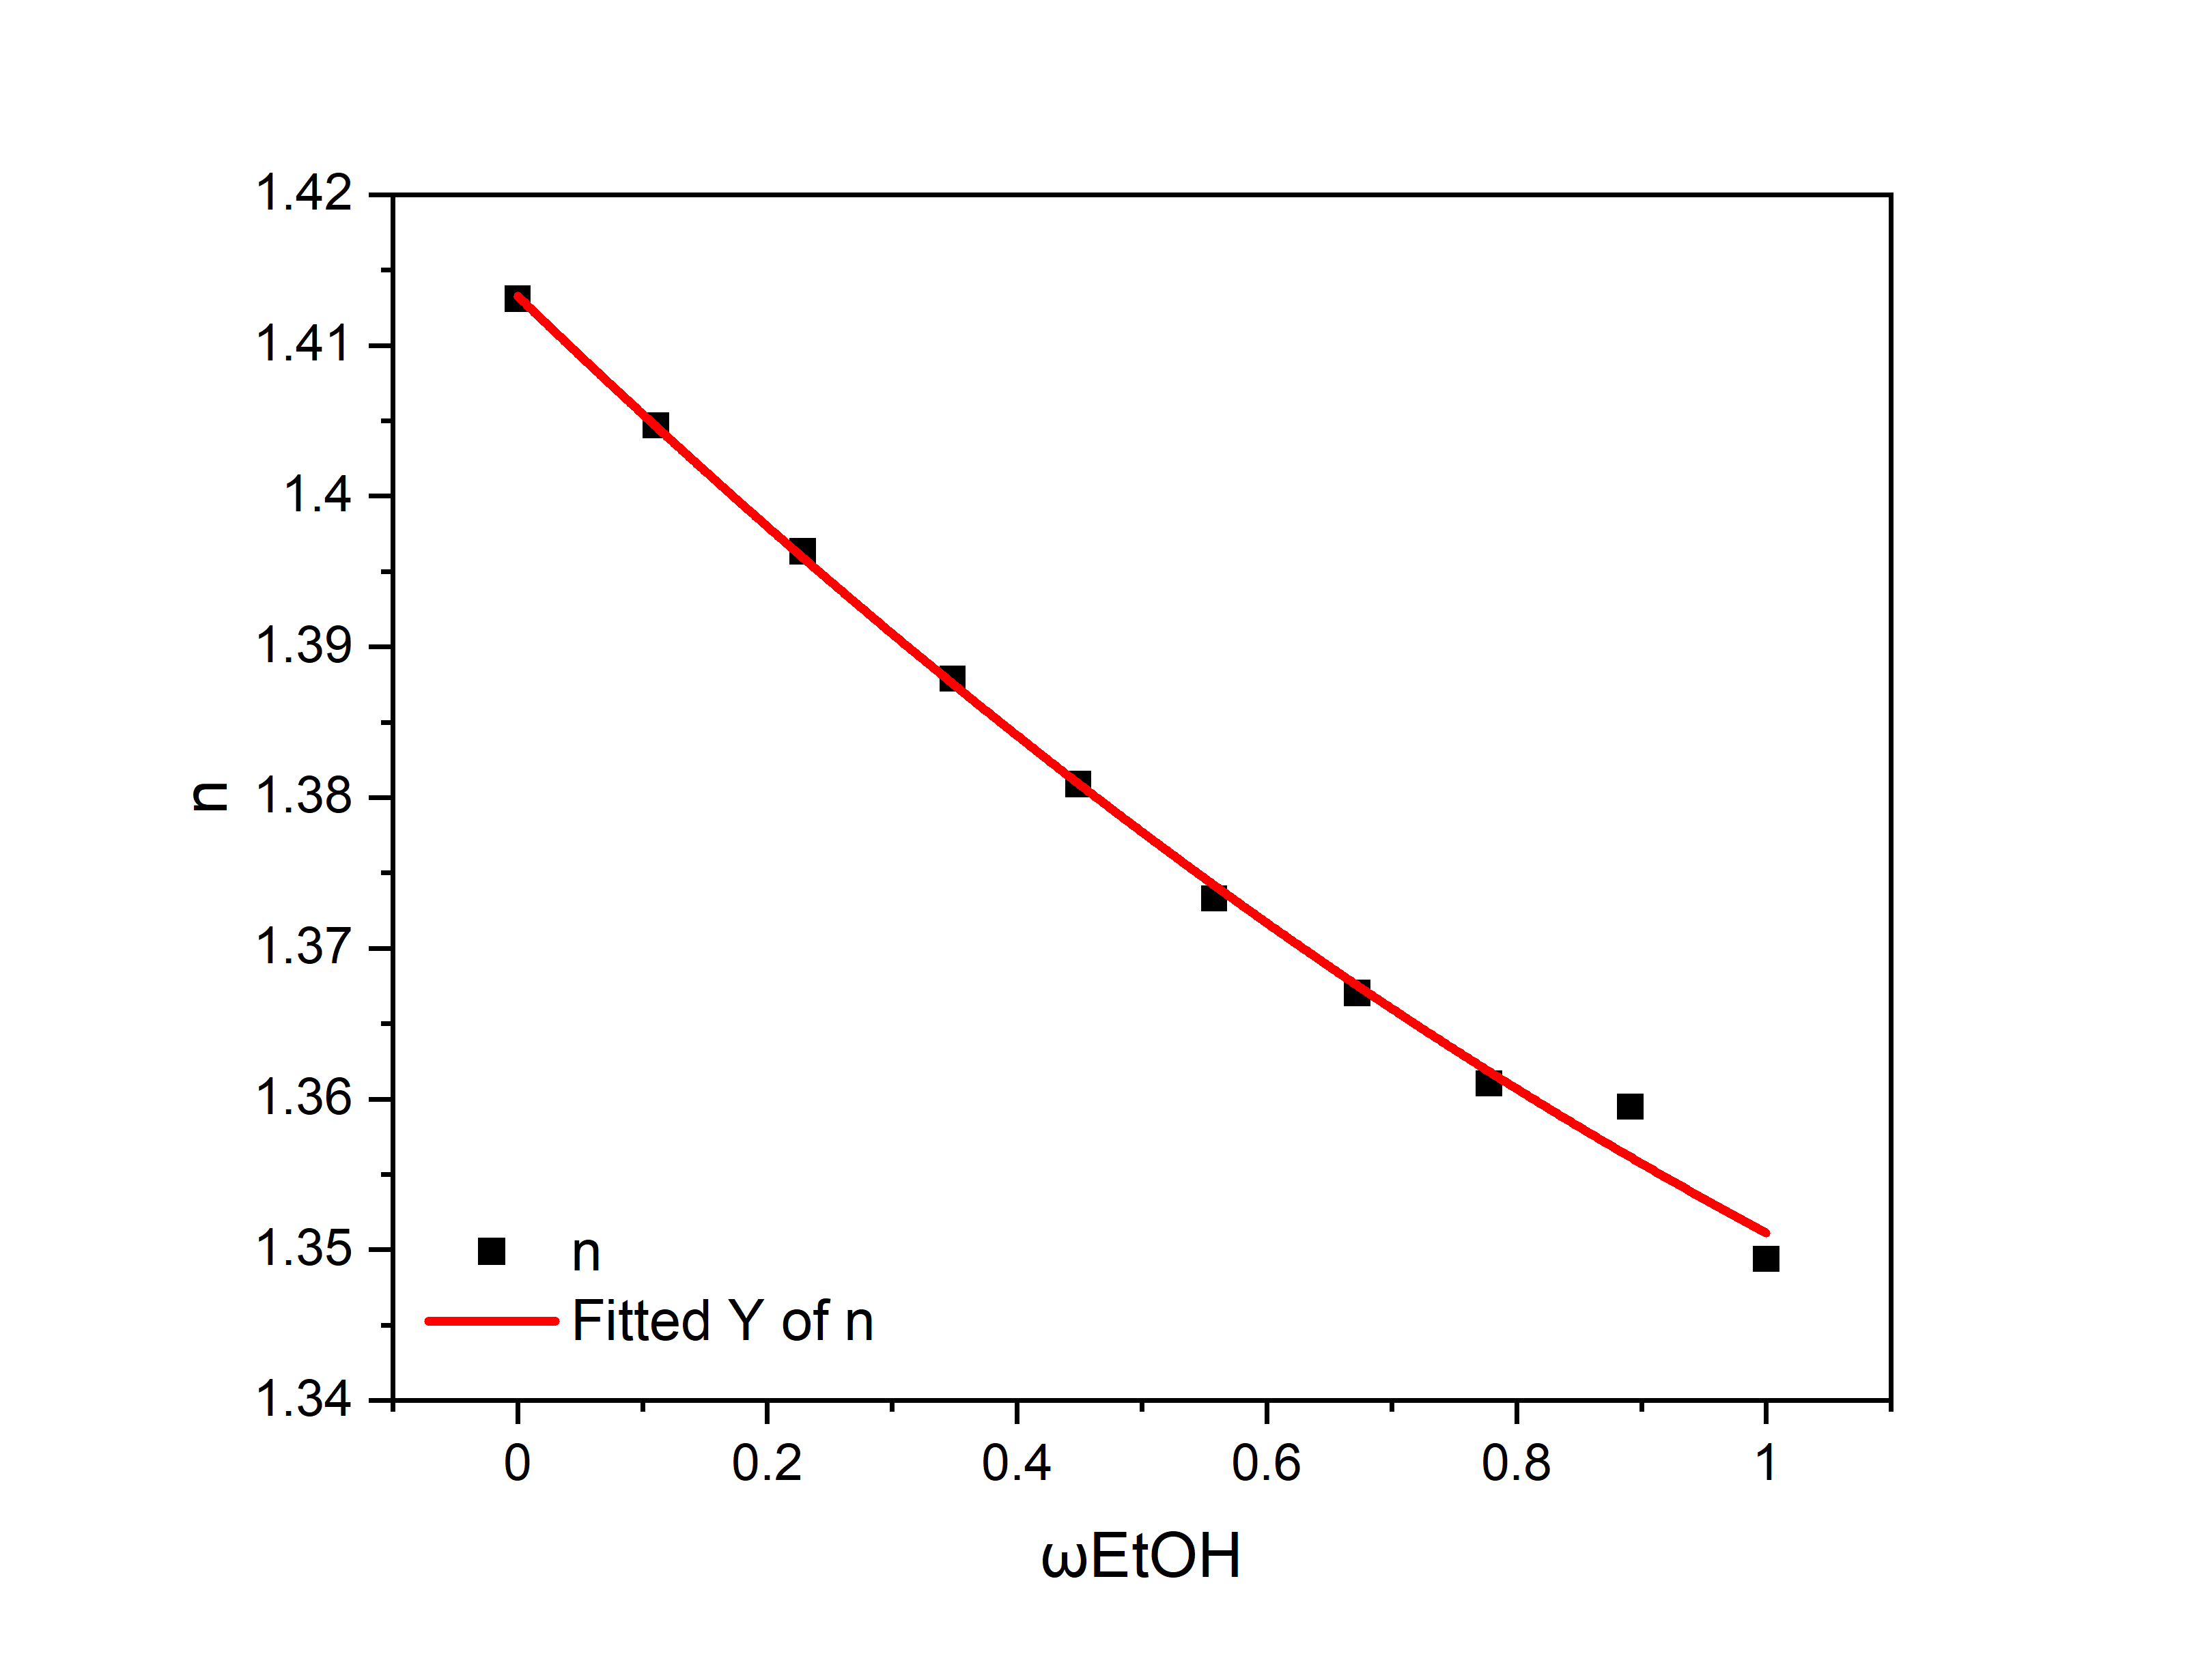
\includegraphics[width = .70\textwidth]{image/Graph3.png}
    \caption{标准溶液的质量分数与折射率的关系}\label{3}
\end{figure}

观察图像发现,在$\omega_{\rm EtOH} = 0.9$附近存在离群值,偏离了拟合曲线较大,同时我们观察残差图 \ref{r} ,可以得到一致的结论。因此我们剔除离群值后再次进行回归得到图像
如图 \ref{4} ,拟合曲线方程如下
$$
\bar{n} =   (1.4133 \pm 0.0003) + (-0.078 \pm 0.001) \cdot \omega_{\rm EtOH} + (0.015 \pm 0.001) \cdot \omega_{\rm EtOH} ^2 \quad R^2 = 0.9998
$$

可以看出乙醇的质量分数与折射率有较好的二次曲线关系,$R^2$ 为0.9998。离群值的出现可能是由于配制溶液出现的误差,以及测量时加入溶液速度较慢造成的误差导致。
观察前后的拟合曲线方程,可以看出对曲线方程的影响并不大,但是显著降低了参数的误差并提高了 $R^2$ 值,因此选择使用剔除后的方程。


\begin{figure}[htbp]
    \centering
    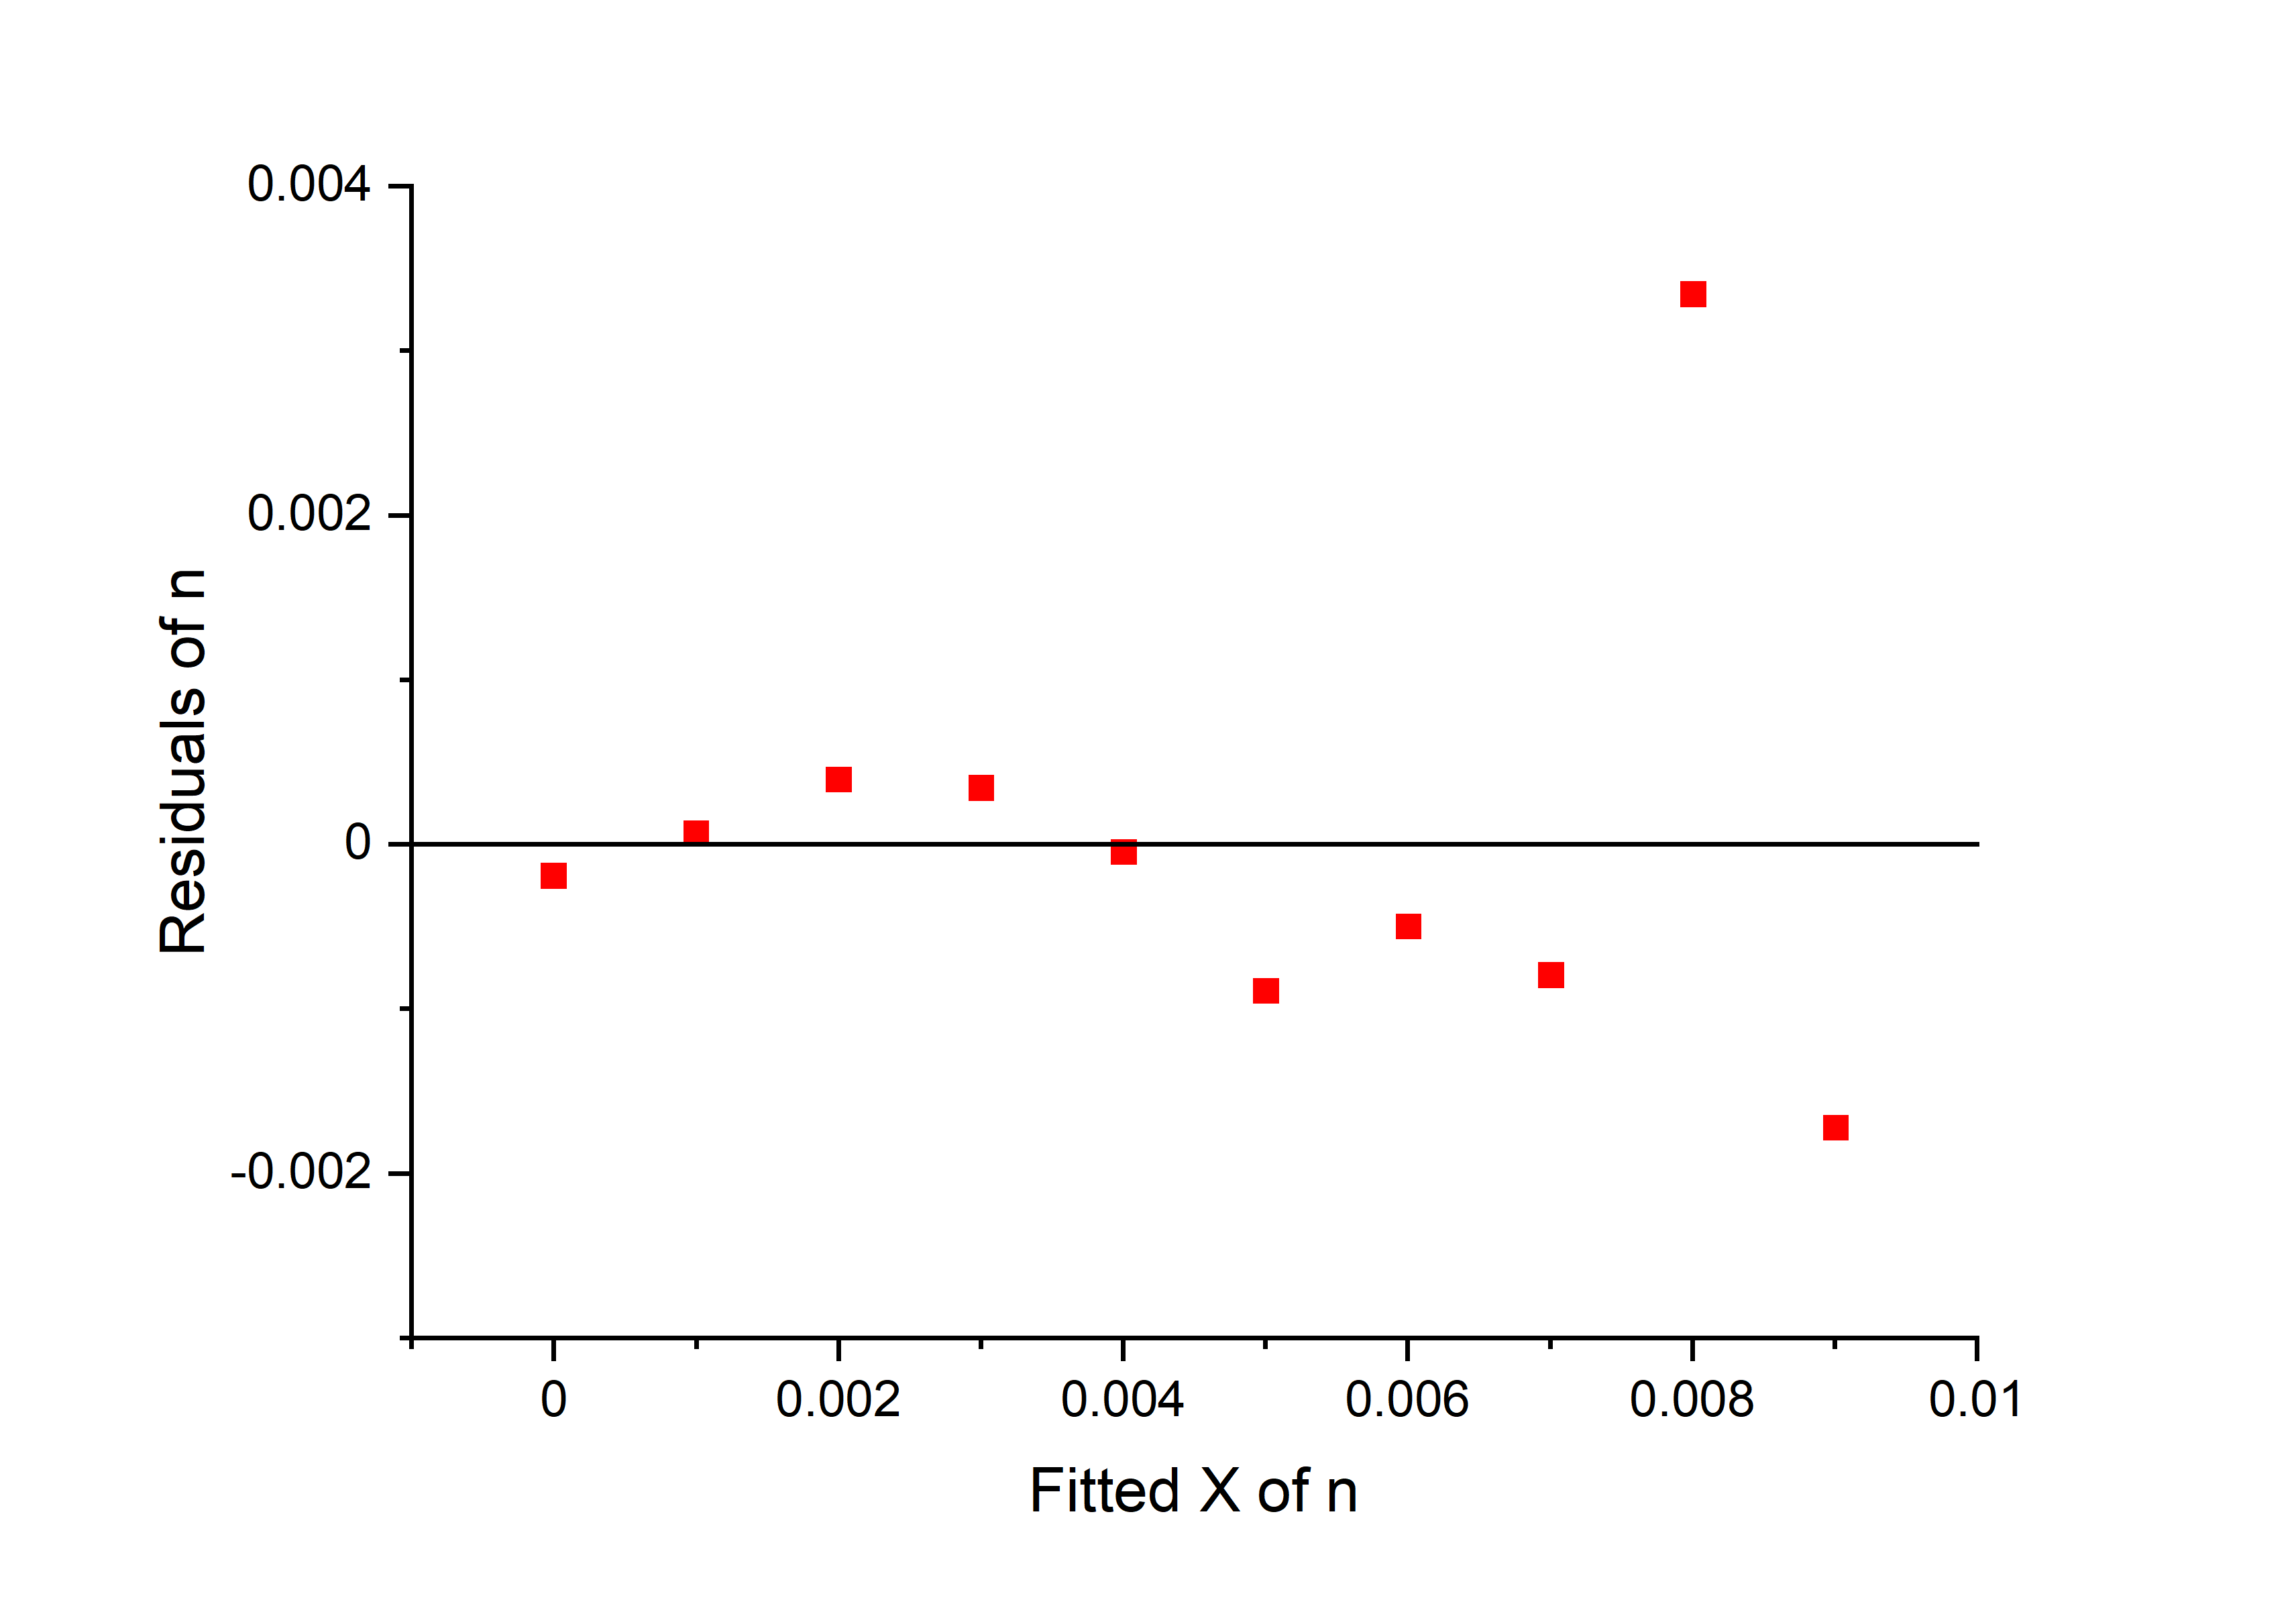
\includegraphics[width = .70\textwidth]{image/Res1.png}
    \caption{标准溶液的质量分数与折射率的关系的残差图}\label{r}
\end{figure}

\begin{figure}[htbp]
    \centering
    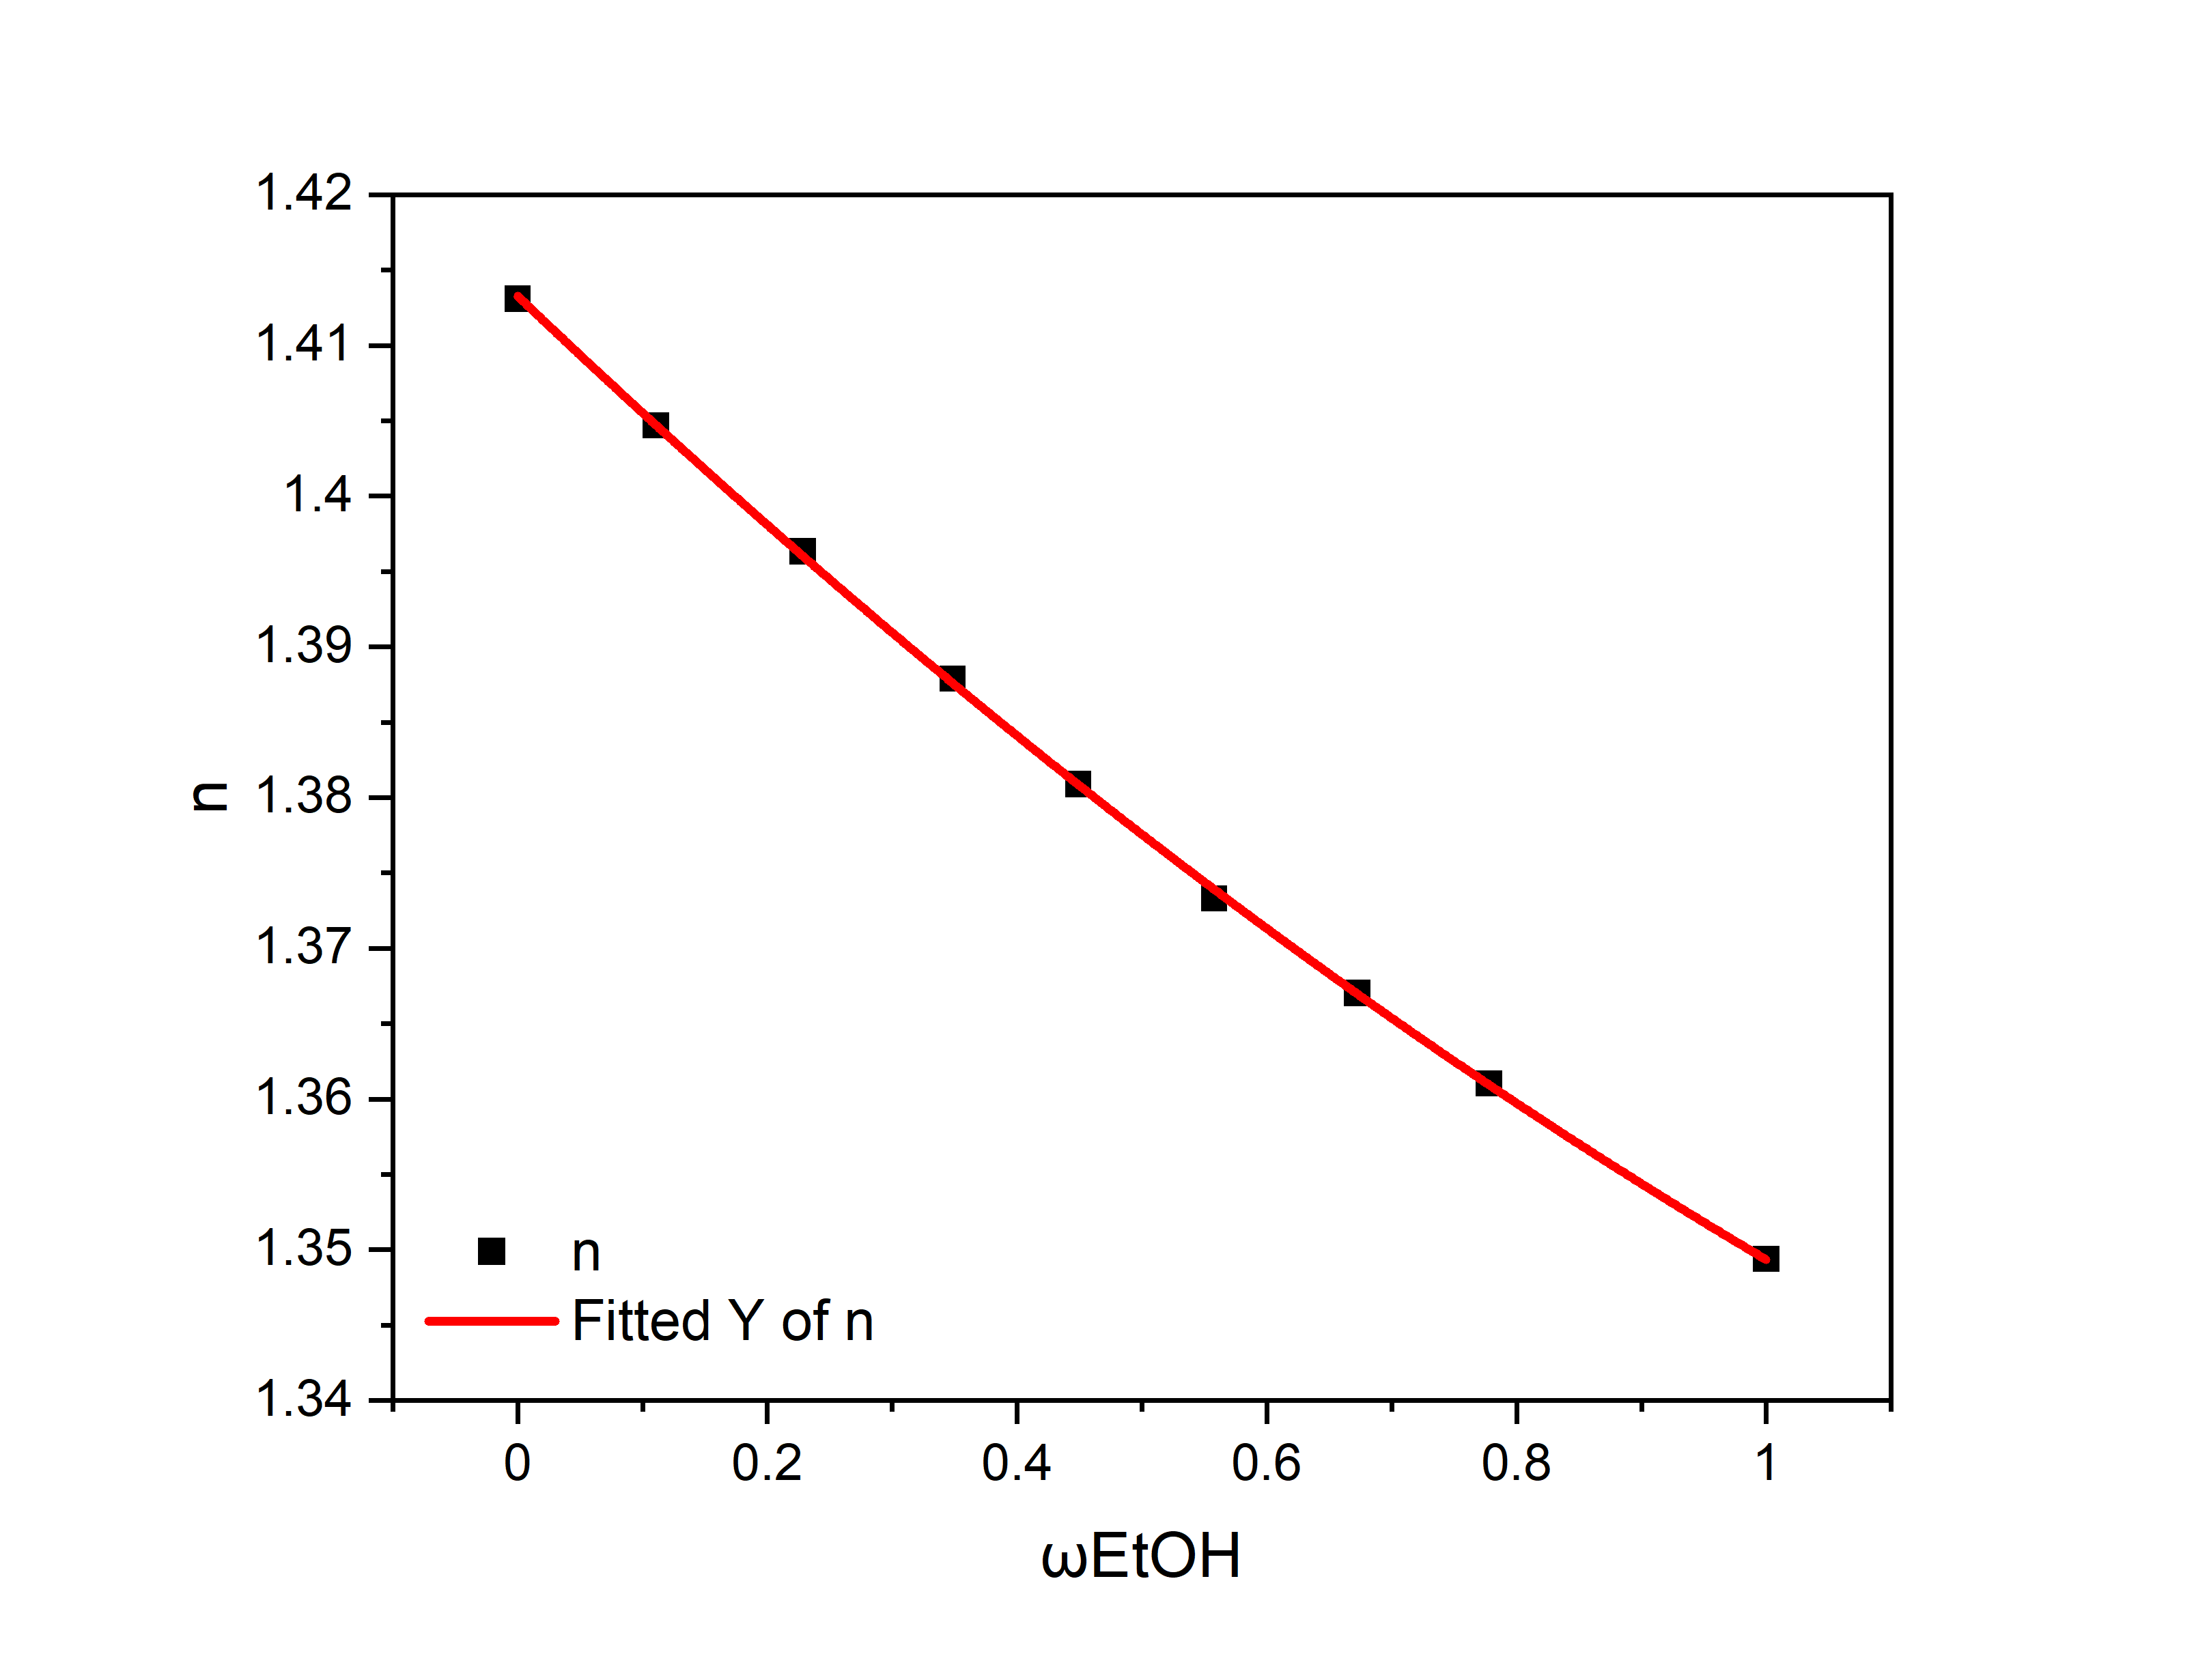
\includegraphics[width = .70\textwidth]{image/Graph4.png}
    \caption{标准溶液的质量分数与折射率的关系(剔除离群值)}\label{4}
\end{figure}

\newpage

\subsection[short]{测定沸点与两相成分}

    测定乙醇-环己烷体系的沸点、冷凝液与恒沸液的折射率如表 \ref{03}。在实验中,由于气相凝结的液体有限,测定三次会带来较大的困难,并且多次测量时溶液再次平衡会带来较大的误差。
    我们采用每一组测定两组气相与液相溶液的旋光度数据的方法。

    根据标准曲线方程,可以计算得到冷凝液与恒沸液的质量分数如表 \ref{05}。

\begin{table}[h]
    \centering
    \caption{乙醇-环己烷的恒沸点和气液两相折射率的测量结果}
    \label{04}
    \begin{tabular}{ccccccccc}
    \hline
    $V_{EtOH}$/mL & $V_{Cy}$/mL & $n_{(l),1}$ & $n_{(l),2}$ & $\bar{n_{(l)}}$ & $n_{(g),1}$ & $n_{(g),2}$ & $\bar{n_{(g)}}$ & bp/$\rm \degree C$ \\ \hline
    20   & 0  & 1.3494 & 1.3495 & 1.3495 & 1.3495 & 1.3496 & 1.3496 & 76.95 \\
    20   & 1  & 1.3515 & 1.3509 & 1.3512 & 1.3675 & 1.3680 & 1.3678 & 73.90 \\
    20   & 2  & 1.3532 & 1.3528 & 1.3530 & 1.3760 & 1.3765 & 1.3763 & 72.30 \\
    20   & 4  & 1.3566 & 1.3570 & 1.3568 & 1.3802 & 1.3800 & 1.3801 & 68.93 \\
    20   & 7  & 1.3630 & 1.3635 & 1.3633 & 1.3865 & 1.3860 & 1.3863 & 66.86 \\
    20   & 10 & 1.3677 & 1.3678 & 1.3678 & 1.3870 & 1.3870 & 1.3870 & 65.71 \\
    20   & 14 & 1.3729 & 1.3729 & 1.3729 & 1.3885 & 1.3885 & 1.3885 & 65.37 \\
    20   & 19 & 1.3795 & 1.3792 & 1.3794 & 1.3896 & 1.3896 & 1.3896 & 64.77 \\
    0    & 20 & 1.4125 & 1.4126 & 1.4126 & 1.4125 & 1.4127 & 1.4126 & 79.62 \\
    0.2  & 20 & 1.4130 & 1.4130 & 1.4130 & 1.3912 & 1.3912 & 1.3912 & 77.32 \\
    0.4  & 20 & 1.4129 & 1.4130 & 1.4130 & 1.3905 & 1.3910 & 1.3908 & 73.99 \\
    0.9  & 20 & 1.4105 & 1.4110 & 1.4108 & 1.3906 & 1.3907 & 1.3907 & 67.49 \\
    1.4  & 20 & 1.4100 & 1.4102 & 1.4101 & 1.3905 & 1.3906 & 1.3906 & 64.94 \\
    3.4  & 20 & 1.4120 & 1.4125 & 1.4123 & 1.3905 & 1.3906 & 1.3906 & 64.51 \\
    8.4  & 20 & 1.3900 & 1.3900 & 1.3900 & 1.3897 & 1.3900 & 1.3899 & 64.34 \\
    13.4 & 20 & 1.3825 & 1.3824 & 1.3825 & 1.3900 & 1.3902 & 1.3901 & 64.31 \\ \hline
    \end{tabular}
\end{table}

\begin{table}[]
    \centering
    \caption{气、液相中乙醇的质量分数与沸点}
    \label{05}
    \begin{tabular}{cccccc}
    \hline
    bp/$\rm \degree C$ & $\omega_{EtOH,l}$ & $\omega_{EtOH,g}$ & bp/$\rm \degree C$ & $\omega_{EtOH,l}$ & $\omega_{EtOH,g}$ \\ \hline
    76.95 & 0.998 & 0.996 & 64.31 & 0.425 & 0.312 \\
    73.90 & 0.963 & 0.660 & 64.34 & 0.314 & 0.316 \\
    72.30 & 0.927 & 0.521 & 64.51 & 0.013 & 0.306 \\
    68.93 & 0.854 & 0.461 & 64.94 & 0.041 & 0.306 \\
    66.86 & 0.737 & 0.368 & 67.49 & 0.032 & 0.304 \\
    65.71 & 0.660 & 0.357 & 73.99 & 0.004 & 0.303 \\
    65.37 & 0.574 & 0.335 & 77.32 & 0.004 & 0.297 \\
    64.77 & 0.472 & 0.320 & 79.62 & 0.009 & 0.009 \\ \hline
    \end{tabular}
\end{table}

\subsection[short]{绘制沸点-两相成分图}

使用表 \ref{05} 的数据绘制沸点-两相成分图,以乙醇质量分数为横坐标,温度为纵坐标作图,用贝塞尔样条曲线(B-spline)进行拟合如图 \ref{7} 。

\begin{figure}[htbp]
    \centering
    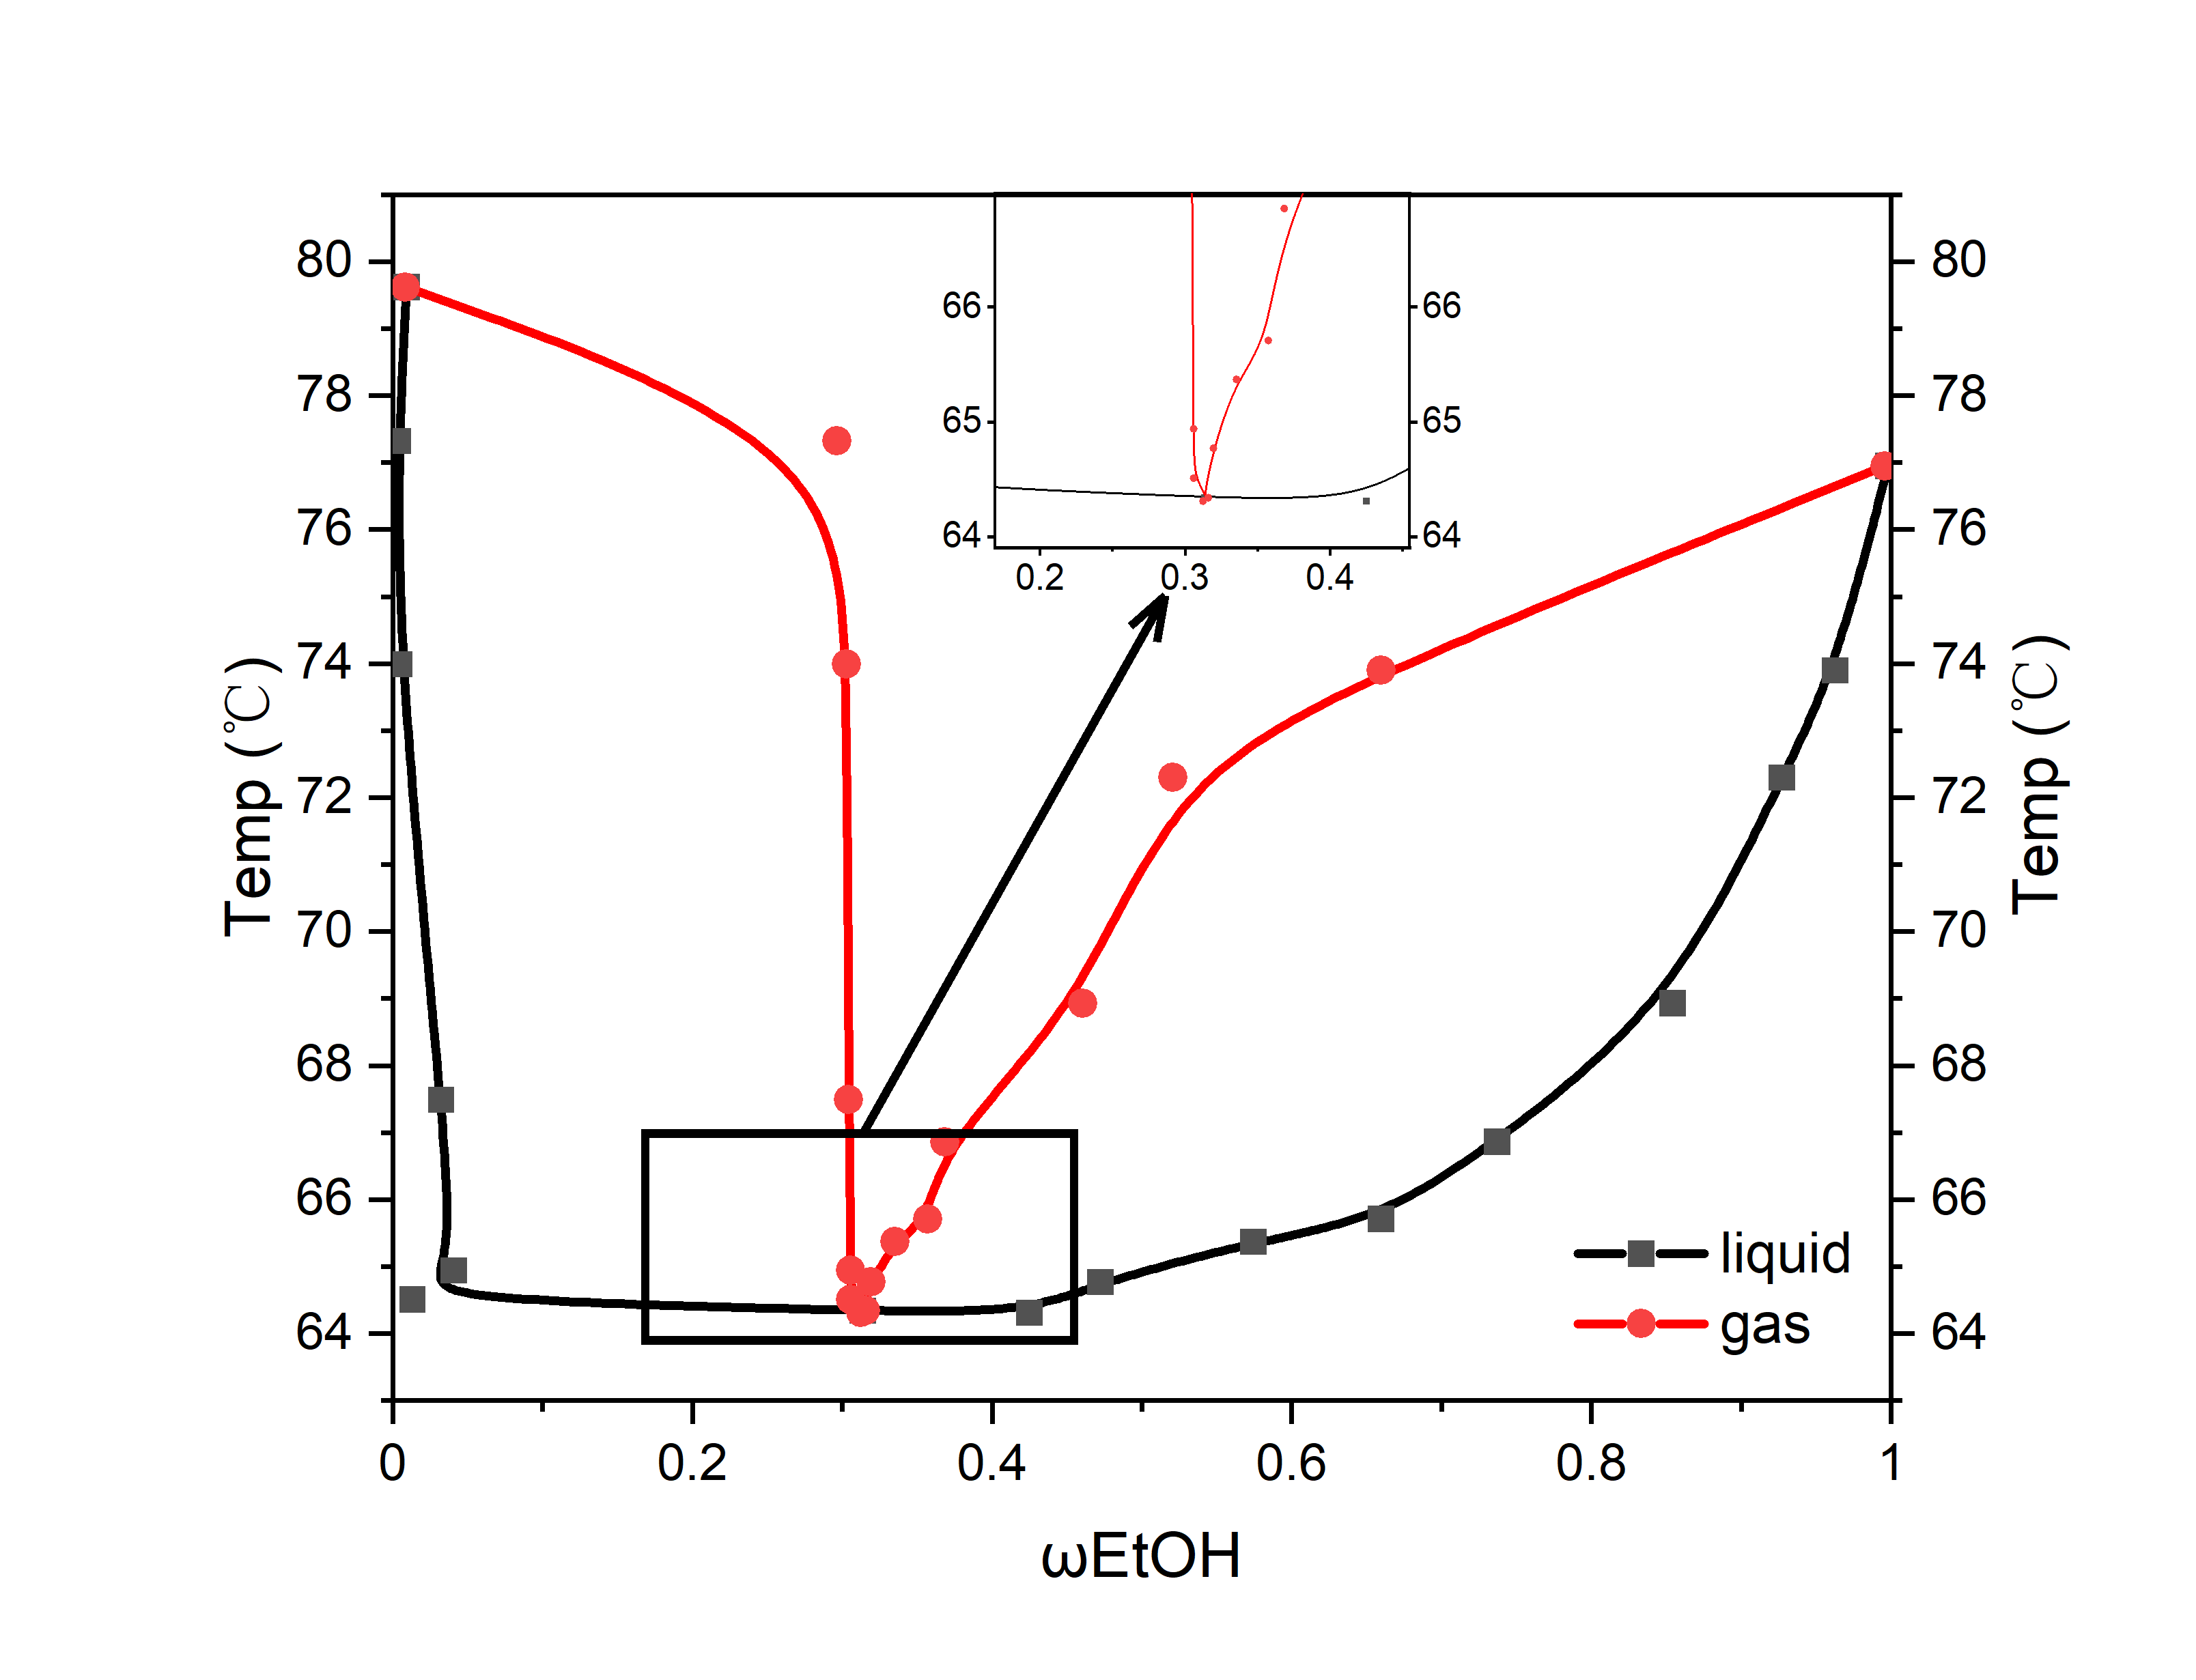
\includegraphics[width = .70\textwidth]{image/Graph8.png}
    \caption{乙醇-环己烷双液体系沸点-两相成分图}\label{7}
\end{figure}

从图中可以看出,该体系的最低恒沸点为:
$$\rm 
T = 64.31 \degree C \quad \omega_{EtOH} = 31.23 \%
$$

根据文献\cite{r},在压强 102.26 kPa 下,EtOH-环己烷的双液体系的最低恒沸点为 64.80 $\degree C
$,此时乙醇的摩尔分数为 0.4540,由此可以计算得到乙醇的质量分数为 0.3128。
因此,实验测得的最低恒沸点与文献值较为吻合。

观察图像可以看到,曲线右侧沸点温度并不随着乙醇液相质量分数上升单调下降,可能的原因是每次测定时取出气相与液相的溶液时间不能保证相同,
且此时液相十分接近纯环己烷,但是同沸点下气相的溶液环己烷质量分数较低,取出气相溶液时就消耗了大部分加入溶液中的乙醇,并且旋光仪的误差
也会显著影响接近纯相溶液的质量分数测定,因此会出现如上的现象。

\section{实验结果与讨论}

\subsection{讨论}

标准溶液经过多人的多次测量,可能会出现溶剂的挥发,导致实验数据准确性不佳。因此我们对比了标准溶液在使用前与使用后的旋光度
结果如下表所示。我们可以看出使用前后的旋光度之差均小于0.0006,说明标准溶液在使用过程中挥发造成的误差较小,因此可以忽略这种误差的影响。

\begin{table}[h]
    \centering
    \caption{标准溶液在使用前与使用后的旋光度}
    \label{06}
    \begin{tabular}{cccc}
    \hline
      & $n_{before}$ & $n_{after}$ & $\Delta n$ \\ \hline
    1 & 1.4133       & 1.4130      & 0.0003     \\
    2 & 1.3985       & 1.3984      & 0.0001     \\
    3 & 1.3957       & 1.3955      & 0.0002     \\
    4 & 1.3890       & 1.3890      & 0.0000     \\
    5 & 1.3735       & 1.3733      & 0.0002     \\
    6 & 1.3745       & 1.3739      & 0.0006     \\
    7 & 1.3683       & 1.3689      & 0.0006     \\
    8 & 1.3630       & 1.3629      & 0.0001     \\ \hline
    \end{tabular}
\end{table}

另外,注意到其他试验台人所测量得到的标准溶液数据与本实验报告中有较大的出入,这是由于不同实验台的仪器的系统误差造成的。
因此不能直接挪用其他试验台的测量数据与工作曲线测量质量分数与绘制相图。


\subsection{结论}

本实验通过配制不同浓度的乙醇-环己烷的标准溶液,通过阿贝折射仪测量溶液的折射率,
绘制乙醇-环己烷体系的折射率-质量分数工作曲线,
并通过测量不同质量分数的乙醇-环己烷恒
沸体系气相和液相的折射率从而确定其质量分数,绘制了乙醇-环己烷双液系的相图,
求得这个体系的最低恒沸点为 64.31 $\rm \degree C$,对应的乙醇的质量分数为 0.3123,与文献值接近。


\nocite{*}
\bibliography{reference}
\end{document}
